\subsection{Frontend}

\subsubsection{Hiện thực Frontend}

\textbf{Kiến trúc phát triển theo tính năng (Feature-based Architecture)}

Mã nguồn Frontend được tổ chức theo mô hình module hóa dựa trên các tính năng nghiệp vụ chính (features). Cách tiếp cận này giúp tách biệt logic của từng thành phần, dễ dàng mở rộng và giảm thiểu xung đột khi nhiều thành viên cùng tham gia phát triển. Mỗi tính năng (như \texttt{auth}, \texttt{product}, \texttt{cart}, \texttt{order}, \texttt{chat-ai}) bao gồm:
\begin{itemize}
    \item \textbf{Components:} Các thành phần giao diện đặc thù cho tính năng đó.
    \item \textbf{Store/Hooks:} Quản lý trạng thái và logic xử lý dữ liệu riêng biệt.
    \item \textbf{API/Services:} Định nghĩa các lời gọi API tới lớp BFF.
\end{itemize}

\textbf{Hiện thực hóa lớp BFF (Backend for Frontend)}

Hệ thống sử dụng Next.js Route Handlers để xây dựng một lớp proxy trung gian. Các yêu cầu từ phía Client (trình duyệt) sẽ được gửi tới các API nội bộ của Next.js, sau đó Route Handlers sẽ chịu trách nhiệm:
\begin{itemize}
    \item Gắn các thông tin định danh (JWT Token) vào header trước khi gửi tới API Gateway.
    \item Hợp nhất dữ liệu từ nhiều dịch vụ khác nhau để giảm số lượng request từ client.
    \item Xử lý lỗi tập trung và trả về mã lỗi chuẩn hóa cho giao diện.
\end{itemize}

\textbf{Tích hợp luồng phản hồi hội thoại AI (Streaming Response)}

Để mang lại trải nghiệm Trợ lý Ảo giống thực tế nhất, nhóm hiện thực cơ chế streaming bằng Vercel AI SDK. Khi người dùng gửi câu hỏi, Frontend sẽ thiết lập một kết nối bất đồng bộ tới AI Agent Service. Dữ liệu trả về dưới dạng dòng văn bản (Server-Sent Events), cho phép UI cập nhật nội dung ngay khi từng từ (token) được tạo ra, thay vì phải chờ đợi toàn bộ câu trả lời hoàn tất.

\subsubsection{Triển khai Frontend}

Frontend của hệ thống được triển khai trên nền tảng \textbf{Vercel}, một cơ sở hạ tầng tối ưu cho các ứng dụng Next.js.

\textbf{Quy trình CI/CD tự động}

Nhóm thiết lập quy trình tích hợp và triển khai liên tục (CI/CD) thông qua việc kết nối kho lưu trữ GitHub với dự án trên Vercel:
\begin{itemize}
    \item \textbf{Tích hợp (CI):} Mỗi khi có một Pull Request mới, hệ thống tự động khởi chạy quy trình kiểm tra mã nguồn (Linting), kiểm tra kiểu (Type Checking) và chạy các bộ Unit Test bằng Vitest.
    \item \textbf{Triển khai (CD):} Sau khi các bài kiểm tra vượt qua và mã nguồn được merge vào nhánh chính (\texttt{main}), Vercel sẽ tự động thực hiện quá trình build và deploy phiên bản mới nhất lên môi trường Production.
\end{itemize}

\begin{figure}[H]
    \centering
    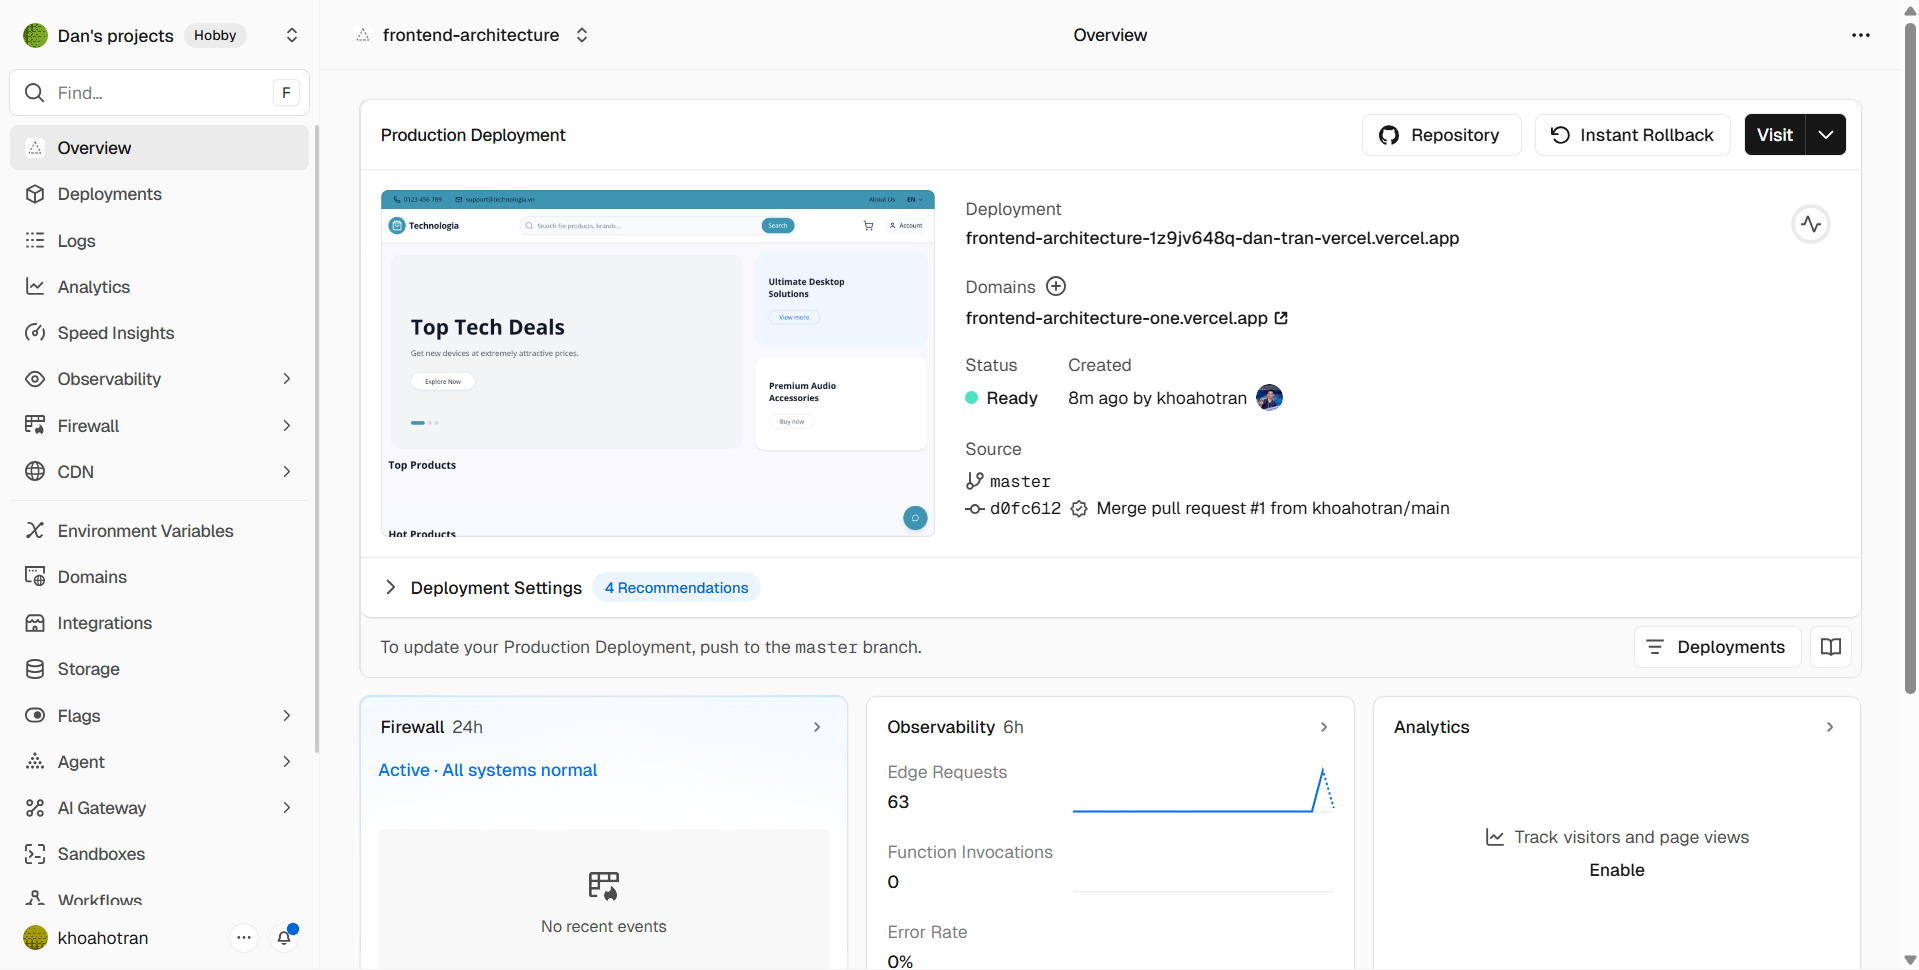
\includegraphics[width=0.95\textwidth]{images/chap7/deployment/vercel_dashboard.png}
    \caption{Trạng thái triển khai và quản lý dự án trên Dashboard của Vercel}
    \label{fig:vercel_deploy}
\end{figure}

\textbf{Tối ưu hóa hiệu năng và bảo mật}

\begin{itemize}
    \item \textbf{Edge Network \& CDN:} Vercel tự động phân phối nội dung tĩnh và render Server Components tại các máy chủ gần người dùng nhất (Edge), giúp giảm thiểu độ trễ.
    \item \textbf{Environment Variables Management:} Các thông tin cấu hình nhạy cảm như URL của API Gateway hay các khóa bí mật được quản lý tập trung trong bảng điều khiển của Vercel, đảm bảo không bị lộ ra ngoài mã nguồn công khai.
    \item \textbf{Analytics \& Monitoring:} Hệ thống tận dụng Vercel Analytics để theo dõi các chỉ số Web Vitals (LCP, FID, CLS), từ đó liên tục tối ưu hóa trải nghiệm người dùng.
\end{itemize}

\begin{figure}[H]
    \centering
    \begin{minipage}{0.48\textwidth}
        \centering
        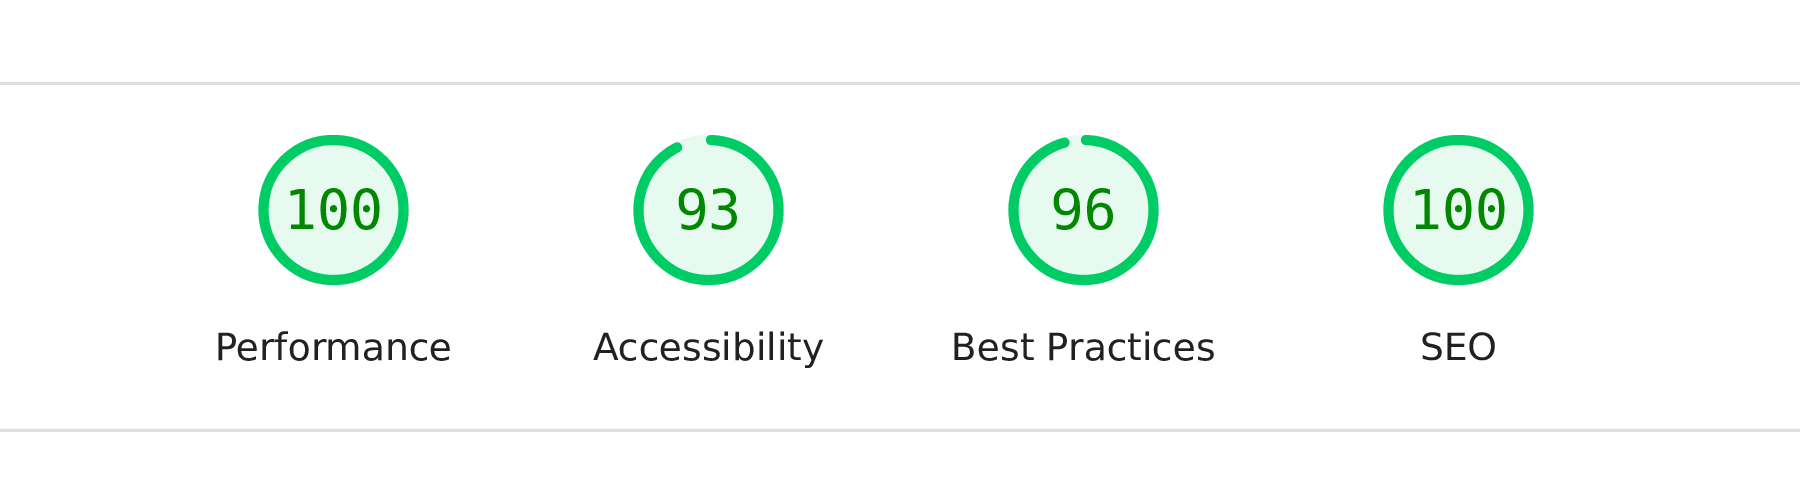
\includegraphics[width=\textwidth]{images/chap7/performance/lh_desktop.png}
        \caption{Chỉ số Lighthouse (Desktop)}
    \end{minipage}
    \hfill
    \begin{minipage}{0.48\textwidth}
        \centering
        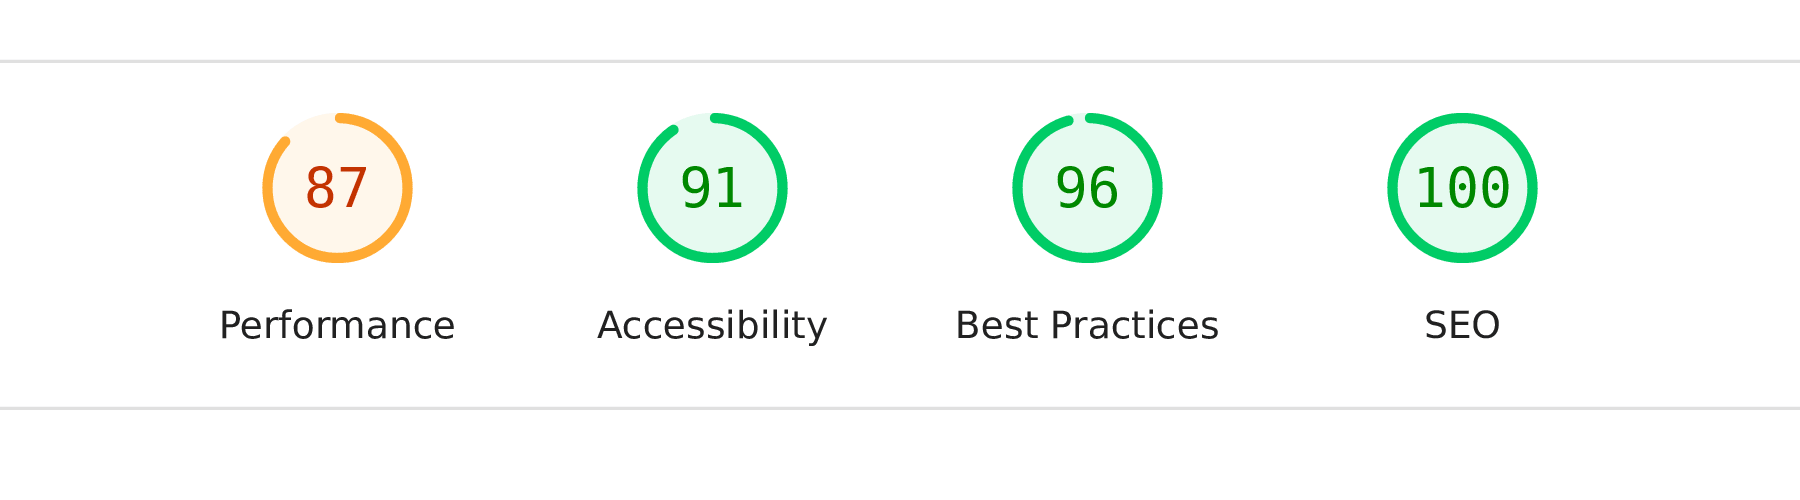
\includegraphics[width=\textwidth]{images/chap7/performance/lh_mobile.png}
        \caption{Chỉ số Lighthouse (Mobile)}
    \end{minipage}
    \label{fig:lighthouse_mini}
\end{figure}
